The training part contains six methods.

\begin{Code}
---------------------------------- python ----------------------------------
>>> romc.solve_problems(n1,
                        use_bo=False,
                        optimizer_args=None,
                        seed=None)
----------------------------------------------------------------------------                    
\end{Code}

\noindent
This method (a) draws the nuisance variables, (b) defines the
optimisation problems and (c) solves them using either a
gradient-based optimizer or Bayesian optimization. These tasks are
compleed sequentially, as shown in figure~\ref{fig:romc_overview}. The
definition of the optimisation problems is performed by drawing
\code{n_1} integer numbers from a discrete uniform distribution
$u_i \sim \mathcal{U}\{1, 2^{32}-1\}$. Each integer $u_i$ is the seed
used in \pkg{ELFI}'s random simulator. The seed $u_i$ is the
computational analogous of the random variables $\vb_i$, that were
defined in the previous chapter; freezing the \code{seed} absorbs all
the randomness of the simulator transforming it to a deterministic
function. Setting the argument \code{use_bo=True}, chooses the
Bayesian Optimisation scheme for obtaining $\thetab_i^*$. In this
case, apart from obtaining the optimal points $\thetab_i^*$, we also
fit a Gaussian Process (GP) as surrogate model $\hat{d}_i$. In this
scenario, in the following steps, $\hat{d}_i(\thetab)$ will replace
$g_i(\thetab)$ as the distance function.

\begin{Code}
---------------------------------- python ----------------------------------
>>> romc.distance_hist(**kwargs)
----------------------------------------------------------------------------  
\end{Code}

\noindent
This function helps the user decide which threshold $\epsilon$ to
use. It plots a histogram of the distances at the optimal point
$g_i(\thetab_i^*) : \{i = 1, 2, \ldots, n_1\}$ or $d_i^*$ in case
\code{use_bo=True}. The function accepts all keyword arguments and
forwards them to the underlying \code{matplotlib.hist()} function; in
this way the user may customise some properties of the histogram, such
as the number of bins or the range of values.

\begin{Code}
---------------------------------- python ----------------------------------  
>>> romc.estimate_regions(eps_filter,
                          use_surrogate=None,
                          region_args=None,
                          fit_models=False,
                          fit_models_args=None,
                          eps_region=None,
                          eps_cutoff=None)
----------------------------------------------------------------------------
\end{Code}

\noindent
This method constructs a bounding box around the optimal point
$\thetab_i^* : i = 1, 2, \ldots, n_1$ following
Algorithm~\ref{alg:region_construction}. The Hessian matrix is
approximated based on the Jacobian $\hess_i = \jac_i^T \jac_i$. The
eigenvectores are computed using the function
\code{numpy.linalg.eig()}. A check is performed so that the matrix
$\hess_i$ is not singular; if this is the case, the eigenvectors are
set to be the vectors of the standard Euclidean basis i.e.\
$\{ \mathbf{e_1} = (1, 0, \ldots), \mathbf{e_2} = (0,1,0,\ldots),
\text{etc} \}$. The limits of the bounding box are obtained by
repeteadly querying the distance function ($g_i(\thetab)$ or
$\hat{d}(\thetab)$) along the search directions given by $\hess_i$.

\begin{Code}
---------------------------------- python ----------------------------------
>>> romc.fit_posterior(args*)  # training in a single call
>>> romc.visualize_region(i)   # acceptance region
>>> romc.compute_eps(quantile) # estimates eps
----------------------------------------------------------------------------
\end{Code}

\noindent
The function \code{fit_posterior} is a syntactic sugar for applying
\code{solve_problems} and \\ \code{estimate_regions} into a single
step. The function \code{visualize_region} can be used for plotting
the bounding box around the optimal point, when the parameter space is
$1D$ or $2D$. The argument \code{i} is the index of the corresponding
optimization problem i.e.\ $i<n_1$. \code{compute_eps} returns the
appropriate distance value $d_{i=\kappa}^*$ where
$\kappa = \lfloor \frac{quantile}{n} \rfloor$ from the collection
$\{ d_i^* \} \forall i = \{1, \ldots, n\}$ where $n$ is the number of
accepted solutions. It can be used to automate the selection of the
threshold $\epsilon$, e.g.\ \code{eps=romc.compute_eps(quantile=0.9)}.


\subsubsection*{Example}


In the following snippet, we put together the routines described above
to perform the training part at our running example.

\begin{Code}
------------------------------ python snippet ------------------------------
  # Trainining (fitting) part
  n1 = 500 # number of optimisation problems
  seed = 21 # seed for solving the optimisation problems
  eps = .75 
  use_bo = False # set to True for switching to Bayesian optimisation

  # Training step-by-step
  romc.solve_problems(n1=n1, seed=seed, use_bo=use_bo)
  romc.theta_hist(bins=100) # plot hist to decide which eps to use

  eps = .75 # threshold for the bounding box based on histogram inspection
  romc.estimate_regions(eps=eps) # build the bounding boxes

  romc.visualize_region(i=1) # for inspecting visually the bounding box

  # Equivalent one-line command
  # romc.fit_posterior(n1=n1, eps=eps, use_bo=use_bo, seed=seed)
----------------------------------------------------------------------------  
\end{Code}

In figure \ref{fig:example_training_hist} we illustrate the
distribution of the distances obtained and the acceptance area of the
first optimisation problem. We observe that most optimal points
produce almost zero distance.

% \begin{figure}[h]
%   \begin{center}
%     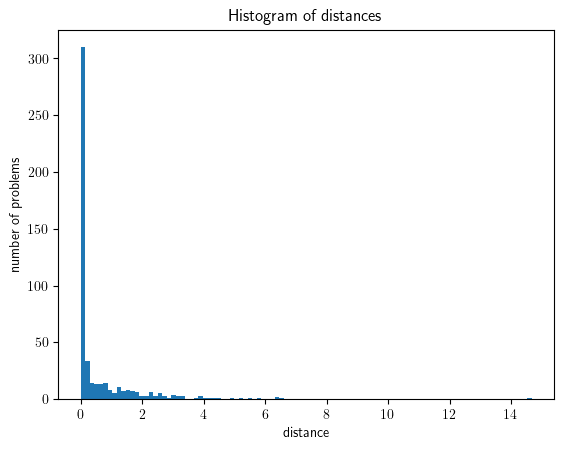
\includegraphics[width=0.48\textwidth]{./latex_files/images/chapter3/example_theta_dist.png}
%     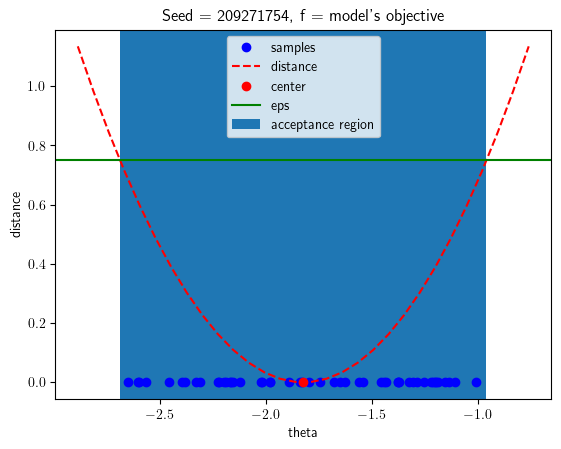
\includegraphics[width=0.48\textwidth]{./latex_files/images/chapter3/example_region_samples.png}
%     \end{center}
%     \caption[Histogram of distances at the 1D example.]{Histogram of
%       distances and visualisation of a specific region.}
%     \label{fig:example_training_hist}
% \end{figure}


% \begin{figure}[h]
%   \begin{center}
%     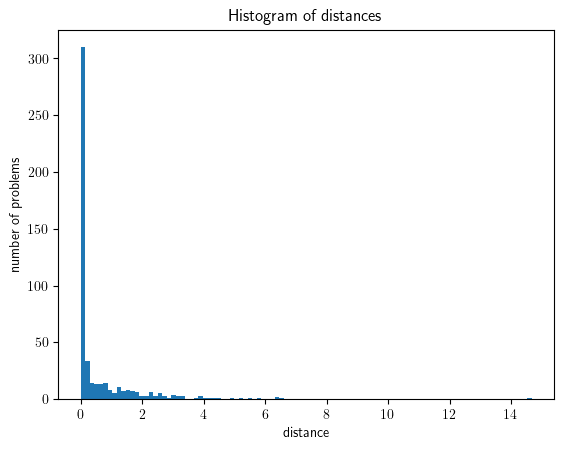
\includegraphics[width=0.32\textwidth]{./latex_files/images/chapter3/example_theta_dist.png}
%     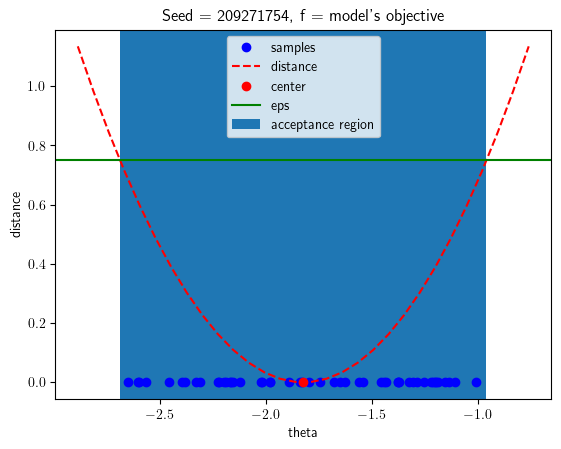
\includegraphics[width=0.32\textwidth]{./latex_files/images/chapter3/example_region_samples.png}
%     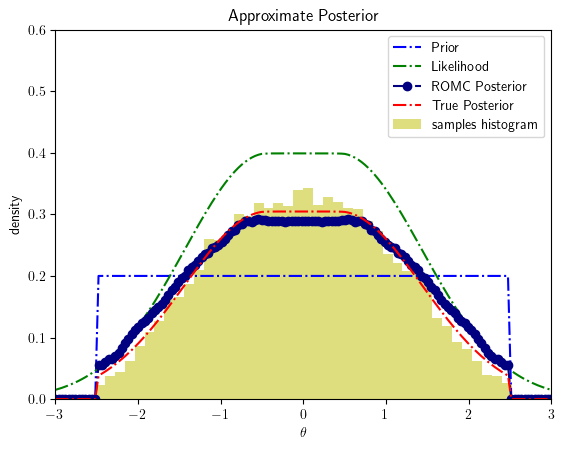
\includegraphics[width=0.32\textwidth]{./latex_files/images/chapter3/example_posterior.png}

%     \end{center}
%     \caption[Histogram of distances at the 1D example.]{Histogram of
%       distances and visualisation of a specific region.}
%     \label{fig:example_training_hist}
%   \end{figure}
  
\begin{figure}[h]
  \begin{center}    
    % This file was created with tikzplotlib v0.9.12.
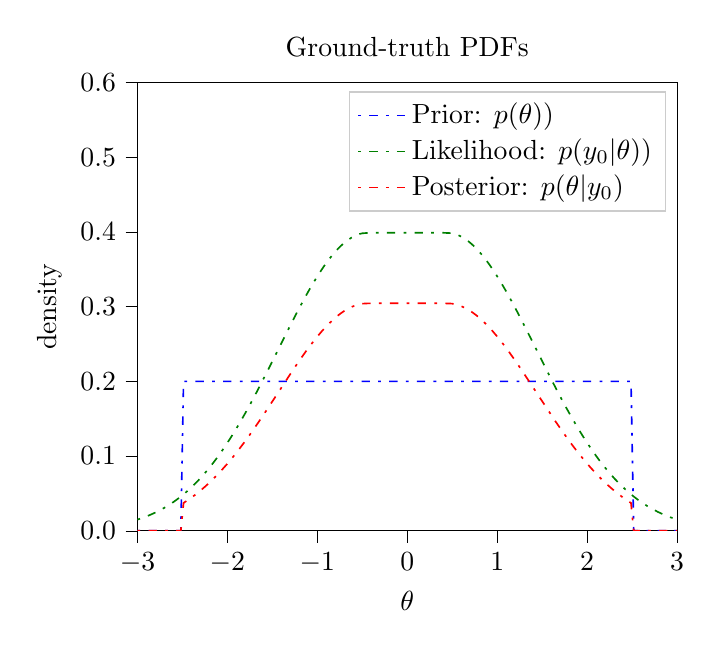
\begin{tikzpicture}

\begin{axis}[
legend cell align={left},
legend style={fill opacity=0.8, draw opacity=1, text opacity=1, draw=white!80!black},
tick align=outside,
tick pos=left,
title={Ground-truth PDFs},
x grid style={white!69.0196078431373!black},
xlabel={\(\displaystyle \theta\)},
xmin=-3, xmax=3,
xtick style={color=black},
xtick={-3,-2,-1,0,1,2,3},
xticklabels={
  \(\displaystyle {\ensuremath{-}3}\),
  \(\displaystyle {\ensuremath{-}2}\),
  \(\displaystyle {\ensuremath{-}1}\),
  \(\displaystyle {0}\),
  \(\displaystyle {1}\),
  \(\displaystyle {2}\),
  \(\displaystyle {3}\)
},
y grid style={white!69.0196078431373!black},
ylabel={density},
ymin=0, ymax=0.6,
ytick style={color=black},
ytick={0,0.1,0.2,0.3,0.4,0.5,0.6},
yticklabels={
  \(\displaystyle {0.0}\),
  \(\displaystyle {0.1}\),
  \(\displaystyle {0.2}\),
  \(\displaystyle {0.3}\),
  \(\displaystyle {0.4}\),
  \(\displaystyle {0.5}\),
  \(\displaystyle {0.6}\)
}
]
\addplot [semithick, blue, dash pattern=on 1pt off 3pt on 3pt off 3pt]
table {%
-3 0
-2.51758790016174 0
-2.48743724822998 0.200000047683716
2.48743724822998 0.200000047683716
2.51758790016174 0
3 0
};
\addlegendentry{Prior: $p(\theta))$}
\addplot [semithick, green!50!black, dash pattern=on 1pt off 3pt on 3pt off 3pt]
table {%
-3 0.0149635076522827
-2.9396984577179 0.0174322128295898
-2.87939691543579 0.0202344655990601
-2.81909537315369 0.0234019756317139
-2.75879406929016 0.0269670486450195
-2.69849252700806 0.030962347984314
-2.63819098472595 0.0354206562042236
-2.57788944244385 0.0403739213943481
-2.51758790016174 0.0458526611328125
-2.45728635787964 0.0518859624862671
-2.39698481559753 0.0584999322891235
-2.33668351173401 0.0657176971435547
-2.2763819694519 0.07355797290802
-2.2160804271698 0.082034707069397
-2.1557788848877 0.0911562442779541
-2.09547734260559 0.100924491882324
-2.03517580032349 0.111333727836609
-1.97487437725067 0.122370958328247
-1.91457283496857 0.134014010429382
-1.85427141189575 0.1462322473526
-1.79396986961365 0.158985257148743
-1.73366832733154 0.172223091125488
-1.67336678504944 0.185885906219482
-1.61306536197662 0.199904561042786
-1.52261304855347 0.221424460411072
-1.28140699863434 0.279423117637634
-1.22110557556152 0.293476581573486
-1.16080403327942 0.30711817741394
-1.10050249099731 0.320227146148682
-1.04020094871521 0.332683801651001
-0.979899525642395 0.344370484352112
-0.949748754501343 0.349889516830444
-0.919597983360291 0.355173826217651
-0.889447212219238 0.360210537910461
-0.859296560287476 0.364986658096313
-0.829145669937134 0.369489908218384
-0.798995018005371 0.373708963394165
-0.768844246864319 0.377632856369019
-0.738693475723267 0.381250977516174
-0.708542704582214 0.384554147720337
-0.678391933441162 0.38753342628479
-0.648241281509399 0.390181064605713
-0.618090391159058 0.392489671707153
-0.587939739227295 0.394453287124634
-0.557788968086243 0.396066427230835
-0.52763819694519 0.397324919700623
-0.497487425804138 0.398194551467896
-0.437186002731323 0.398676156997681
-0.346733689308167 0.398900628089905
-0.0150753259658813 0.398942232131958
0.407035112380981 0.398792028427124
0.467336654663086 0.398488640785217
0.497487425804138 0.398194551467896
0.52763819694519 0.397324919700623
0.557788968086243 0.396066427230835
0.587939739227295 0.394453287124634
0.618090391159058 0.392489671707153
0.648241281509399 0.390181064605713
0.678391933441162 0.38753342628479
0.708542704582214 0.384554147720337
0.738693475723267 0.381250977516174
0.768844246864319 0.377632856369019
0.798995018005371 0.373708963394165
0.829145669937134 0.369489908218384
0.859296560287476 0.364986658096313
0.889447212219238 0.360210537910461
0.919597983360291 0.355173826217651
0.949748754501343 0.349889516830444
0.979899525642395 0.344370484352112
1.04020094871521 0.332683801651001
1.10050249099731 0.320227146148682
1.16080403327942 0.30711817741394
1.22110557556152 0.293476581573486
1.28140699863434 0.279423117637634
1.3718593120575 0.257830619812012
1.58291459083557 0.207022905349731
1.64321613311768 0.192855477333069
1.70351755619049 0.17900550365448
1.7638190984726 0.165547132492065
1.8241206407547 0.152544856071472
1.88442206382751 0.140053510665894
1.94472360610962 0.128118515014648
2.00502514839172 0.116775035858154
2.06532669067383 0.106049656867981
2.12562823295593 0.0959596633911133
2.18592953681946 0.0865145921707153
2.24623107910156 0.0777161121368408
2.30653262138367 0.0695589780807495
2.36683416366577 0.0620321035385132
2.42713570594788 0.0551187992095947
2.48743724822998 0.0487983226776123
2.54773879051208 0.0430457592010498
2.60804009437561 0.0378334522247314
2.66834163665771 0.0331317186355591
2.72864317893982 0.0289088487625122
2.78894472122192 0.0251327753067017
2.84924626350403 0.0217704772949219
2.90954780578613 0.0187896490097046
2.96984934806824 0.0161581039428711
3 0.0149635076522827
};
\addlegendentry{Likelihood: $p(y_0|\theta))$}
\addplot [semithick, red, dash pattern=on 1pt off 3pt on 3pt off 3pt]
table {%
-3 0
-2.51758790016174 0
-2.48743724822998 0.0372545719146729
-2.42713570594788 0.0420799255371094
-2.36683416366577 0.0473577976226807
-2.30653262138367 0.0531041622161865
-2.24623107910156 0.0593316555023193
-2.18592953681946 0.0660487413406372
-2.12562823295593 0.0732594728469849
-2.06532669067383 0.0809625387191772
-2.00502514839172 0.0891507863998413
-1.94472360610962 0.0978107452392578
-1.88442206382751 0.106922507286072
-1.8241206407547 0.116458892822266
-1.7638190984726 0.12638533115387
-1.70351755619049 0.136659979820251
-1.61306536197662 0.152615189552307
-1.52261304855347 0.169044375419617
-1.25125622749329 0.21872091293335
-1.19095480442047 0.229304075241089
-1.13065326213837 0.239526867866516
-1.07035171985626 0.249297142028809
-1.01005029678345 0.258524179458618
-0.949748754501343 0.267119646072388
-0.889447212219238 0.274999141693115
-0.829145669937134 0.282083511352539
-0.798995018005371 0.285304546356201
-0.768844246864319 0.288300037384033
-0.738693475723267 0.291062355041504
-0.708542704582214 0.293584108352661
-0.678391933441162 0.29585862159729
-0.648241281509399 0.297879934310913
-0.618090391159058 0.299642443656921
-0.587939739227295 0.301141500473022
-0.557788968086243 0.302373051643372
-0.52763819694519 0.303333759307861
-0.497487425804138 0.303997755050659
-0.437186002731323 0.304365396499634
-0.316582918167114 0.304553270339966
0.346733689308167 0.304536819458008
0.467336654663086 0.304222345352173
0.497487425804138 0.303997755050659
0.52763819694519 0.303333759307861
0.557788968086243 0.302373051643372
0.587939739227295 0.301141500473022
0.618090391159058 0.299642443656921
0.648241281509399 0.297879934310913
0.678391933441162 0.29585862159729
0.708542704582214 0.293584108352661
0.738693475723267 0.291062355041504
0.768844246864319 0.288300037384033
0.798995018005371 0.285304546356201
0.829145669937134 0.282083511352539
0.889447212219238 0.274999141693115
0.949748754501343 0.267119646072388
1.01005029678345 0.258524179458618
1.07035171985626 0.249297142028809
1.13065326213837 0.239526867866516
1.19095480442047 0.229304075241089
1.25125622749329 0.21872091293335
1.34170854091644 0.202370405197144
1.64321613311768 0.147233605384827
1.73366832733154 0.131482005119324
1.79396986961365 0.121375799179077
1.85427141189575 0.111639618873596
1.91457283496857 0.102311730384827
1.97487437725067 0.0934228897094727
2.03517580032349 0.0849967002868652
2.09547734260559 0.077049732208252
2.1557788848877 0.0695923566818237
2.2160804271698 0.0626286268234253
2.2763819694519 0.056157112121582
2.33668351173401 0.0501714944839478
2.39698481559753 0.044661283493042
2.45728635787964 0.03961181640625
2.48743724822998 0.0372545719146729
2.51758790016174 0
3 0
};
\addlegendentry{Posterior: $p(\theta|y_0)$}
\end{axis}

\end{tikzpicture}

    % This file was created by tikzplotlib v0.9.9.
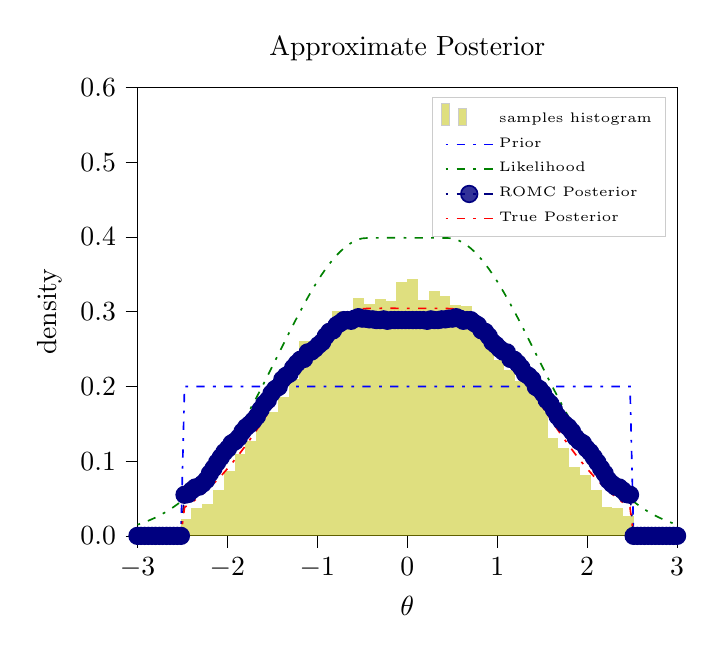
\begin{tikzpicture}

\definecolor{color0}{rgb}{0.75,0.75,0}

\begin{axis}[
legend cell align={left},
legend style={fill opacity=0.8, draw opacity=1, text opacity=1, draw=white!80!black, font=\tiny},
tick align=outside,
tick pos=left,
title={Approximate Posterior},
x grid style={white!69.0196078431373!black},
xlabel={\(\displaystyle \theta\)},
xmin=-3, xmax=3,
xtick style={color=black},
xtick={-3,-2,-1,0,1,2,3},
xticklabels={
  \(\displaystyle {\ensuremath{-}3}\),
  \(\displaystyle {\ensuremath{-}2}\),
  \(\displaystyle {\ensuremath{-}1}\),
  \(\displaystyle {0}\),
  \(\displaystyle {1}\),
  \(\displaystyle {2}\),
  \(\displaystyle {3}\)
},
y grid style={white!69.0196078431373!black},
ylabel={density},
ymin=0, ymax=0.6,
ytick style={color=black},
ytick={0,0.1,0.2,0.3,0.4,0.5,0.6},
yticklabels={
  \(\displaystyle {0.0}\),
  \(\displaystyle {0.1}\),
  \(\displaystyle {0.2}\),
  \(\displaystyle {0.3}\),
  \(\displaystyle {0.4}\),
  \(\displaystyle {0.5}\),
  \(\displaystyle {0.6}\)
}
]
\draw[draw=none,fill=color0,fill opacity=0.5] (axis cs:-3,0) rectangle (axis cs:-2.88,0);
\addlegendimage{ybar,ybar legend,draw=none,fill=color0,fill opacity=0.5}
\addlegendentry{samples histogram}

\draw[draw=none,fill=color0,fill opacity=0.5] (axis cs:-2.88,0) rectangle (axis cs:-2.76,0);
\draw[draw=none,fill=color0,fill opacity=0.5] (axis cs:-2.76,0) rectangle (axis cs:-2.64,0);
\draw[draw=none,fill=color0,fill opacity=0.5] (axis cs:-2.64,0) rectangle (axis cs:-2.52,0);
\draw[draw=none,fill=color0,fill opacity=0.5] (axis cs:-2.52,0) rectangle (axis cs:-2.4,0.0232073945389685);
\draw[draw=none,fill=color0,fill opacity=0.5] (axis cs:-2.4,0) rectangle (axis cs:-2.28,0.0370673662775194);
\draw[draw=none,fill=color0,fill opacity=0.5] (axis cs:-2.28,0) rectangle (axis cs:-2.16,0.0432283769706026);
\draw[draw=none,fill=color0,fill opacity=0.5] (axis cs:-2.16,0) rectangle (axis cs:-2.04,0.0612233170218504);
\draw[draw=none,fill=color0,fill opacity=0.5] (axis cs:-2.04,0) rectangle (axis cs:-1.92,0.0863738703892799);
\draw[draw=none,fill=color0,fill opacity=0.5] (axis cs:-1.92,0) rectangle (axis cs:-1.8,0.109332614272474);
\draw[draw=none,fill=color0,fill opacity=0.5] (axis cs:-1.8,0) rectangle (axis cs:-1.68,0.1270696943844);
\draw[draw=none,fill=color0,fill opacity=0.5] (axis cs:-1.68,0) rectangle (axis cs:-1.56,0.162608319593082);
\draw[draw=none,fill=color0,fill opacity=0.5] (axis cs:-1.56,0) rectangle (axis cs:-1.44,0.165932870953625);
\draw[draw=none,fill=color0,fill opacity=0.5] (axis cs:-1.44,0) rectangle (axis cs:-1.32,0.186184085473939);
\draw[draw=none,fill=color0,fill opacity=0.5] (axis cs:-1.32,0) rectangle (axis cs:-1.2,0.21004533914476);
\draw[draw=none,fill=color0,fill opacity=0.5] (axis cs:-1.2,0) rectangle (axis cs:-1.08,0.260281980894789);
\draw[draw=none,fill=color0,fill opacity=0.5] (axis cs:-1.08,0) rectangle (axis cs:-0.96,0.258872960512065);
\draw[draw=none,fill=color0,fill opacity=0.5] (axis cs:-0.96,0) rectangle (axis cs:-0.84,0.267861221254142);
\draw[draw=none,fill=color0,fill opacity=0.5] (axis cs:-0.84,0) rectangle (axis cs:-0.72,0.301309339097609);
\draw[draw=none,fill=color0,fill opacity=0.5] (axis cs:-0.72,0) rectangle (axis cs:-0.6,0.296677069473362);
\draw[draw=none,fill=color0,fill opacity=0.5] (axis cs:-0.6,0) rectangle (axis cs:-0.48,0.318079444437077);
\draw[draw=none,fill=color0,fill opacity=0.5] (axis cs:-0.48,0) rectangle (axis cs:-0.36,0.310739645449952);
\draw[draw=none,fill=color0,fill opacity=0.5] (axis cs:-0.36,0) rectangle (axis cs:-0.24,0.317600561692622);
\draw[draw=none,fill=color0,fill opacity=0.5] (axis cs:-0.24,0) rectangle (axis cs:-0.12,0.313833964721813);
\draw[draw=none,fill=color0,fill opacity=0.5] (axis cs:-0.12,0) rectangle (axis cs:0,0.340218562084569);
\draw[draw=none,fill=color0,fill opacity=0.5] (axis cs:0,0) rectangle (axis cs:0.12,0.343469439176735);
\draw[draw=none,fill=color0,fill opacity=0.5] (axis cs:0.12,0) rectangle (axis cs:0.24,0.315528472894501);
\draw[draw=none,fill=color0,fill opacity=0.5] (axis cs:0.24,0) rectangle (axis cs:0.36,0.327491332222326);
\draw[draw=none,fill=color0,fill opacity=0.5] (axis cs:0.36,0) rectangle (axis cs:0.48,0.320667253113843);
\draw[draw=none,fill=color0,fill opacity=0.5] (axis cs:0.48,0) rectangle (axis cs:0.6,0.309533229305267);
\draw[draw=none,fill=color0,fill opacity=0.5] (axis cs:0.6,0) rectangle (axis cs:0.72,0.307884767550316);
\draw[draw=none,fill=color0,fill opacity=0.5] (axis cs:0.72,0) rectangle (axis cs:0.84,0.289208340516575);
\draw[draw=none,fill=color0,fill opacity=0.5] (axis cs:0.84,0) rectangle (axis cs:0.96,0.272217212371973);
\draw[draw=none,fill=color0,fill opacity=0.5] (axis cs:0.96,0) rectangle (axis cs:1.08,0.235895798061777);
\draw[draw=none,fill=color0,fill opacity=0.5] (axis cs:1.08,0) rectangle (axis cs:1.2,0.221437222892658);
\draw[draw=none,fill=color0,fill opacity=0.5] (axis cs:1.2,0) rectangle (axis cs:1.32,0.207761436825051);
\draw[draw=none,fill=color0,fill opacity=0.5] (axis cs:1.32,0) rectangle (axis cs:1.44,0.206149812204291);
\draw[draw=none,fill=color0,fill opacity=0.5] (axis cs:1.44,0) rectangle (axis cs:1.56,0.191175517156526);
\draw[draw=none,fill=color0,fill opacity=0.5] (axis cs:1.56,0) rectangle (axis cs:1.68,0.130919174907133);
\draw[draw=none,fill=color0,fill opacity=0.5] (axis cs:1.68,0) rectangle (axis cs:1.8,0.118127480060059);
\draw[draw=none,fill=color0,fill opacity=0.5] (axis cs:1.8,0) rectangle (axis cs:1.92,0.0924796253810799);
\draw[draw=none,fill=color0,fill opacity=0.5] (axis cs:1.92,0) rectangle (axis cs:2.04,0.0812258808863897);
\draw[draw=none,fill=color0,fill opacity=0.5] (axis cs:2.04,0) rectangle (axis cs:2.16,0.0618587575866078);
\draw[draw=none,fill=color0,fill opacity=0.5] (axis cs:2.16,0) rectangle (axis cs:2.28,0.0384119216754122);
\draw[draw=none,fill=color0,fill opacity=0.5] (axis cs:2.28,0) rectangle (axis cs:2.4,0.0377120161258239);
\draw[draw=none,fill=color0,fill opacity=0.5] (axis cs:2.4,0) rectangle (axis cs:2.52,0.026430643780492);
\draw[draw=none,fill=color0,fill opacity=0.5] (axis cs:2.52,0) rectangle (axis cs:2.64,0);
\draw[draw=none,fill=color0,fill opacity=0.5] (axis cs:2.64,0) rectangle (axis cs:2.76,0);
\draw[draw=none,fill=color0,fill opacity=0.5] (axis cs:2.76,0) rectangle (axis cs:2.88,0);
\draw[draw=none,fill=color0,fill opacity=0.5] (axis cs:2.88,0) rectangle (axis cs:3,0);
\addplot [semithick, blue, dash pattern=on 1pt off 3pt on 3pt off 3pt]
table {%
-3 0
-2.51677846908569 0
-2.4765100479126 0.200000047683716
2.4765100479126 0.200000047683716
2.51677846908569 0
3 0
};
\addlegendentry{Prior}
\addplot [semithick, green!50!black, dash pattern=on 1pt off 3pt on 3pt off 3pt]
table {%
-3 0.0149635076522827
-2.91946315765381 0.0183337926864624
-2.83892607688904 0.0223180055618286
-2.75838923454285 0.0269923210144043
-2.67785239219666 0.0324347019195557
-2.63758397102356 0.0354681015014648
-2.59731554985046 0.0387222766876221
-2.55704689025879 0.0422066450119019
-2.51677846908569 0.0459299087524414
-2.4765100479126 0.0499007701873779
-2.4362416267395 0.0541269779205322
-2.39597320556641 0.058616042137146
-2.35570478439331 0.0633745193481445
-2.31543612480164 0.0684083700180054
-2.27516770362854 0.073722243309021
-2.23489928245544 0.0793203115463257
-2.19463086128235 0.0852051973342896
-2.15436244010925 0.0913783311843872
-2.11409401893616 0.0978399515151978
-2.07382559776306 0.104588747024536
-2.03355693817139 0.111621975898743
-1.99328863620758 0.118935108184814
-1.9530200958252 0.126521944999695
-1.9127516746521 0.134374856948853
-1.872483253479 0.142483830451965
-1.83221471309662 0.150837302207947
-1.79194629192352 0.159421920776367
-1.71140944957733 0.177220344543457
-1.63087248802185 0.195732235908508
-1.55033552646637 0.214780211448669
-1.3892617225647 0.253633737564087
-1.30872488021851 0.272953271865845
-1.22818791866302 0.291845083236694
-1.14765095710754 0.310027003288269
-1.10738253593445 0.318762183189392
-1.06711411476135 0.327212452888489
-1.02684569358826 0.335342526435852
-0.986577153205872 0.343117833137512
-0.946308732032776 0.350504517555237
-0.906040191650391 0.357470154762268
-0.865771770477295 0.363983392715454
-0.825503349304199 0.370014905929565
-0.785234928131104 0.375536918640137
-0.744966506958008 0.380523920059204
-0.704697966575623 0.384952306747437
-0.664429545402527 0.388801217079163
-0.624161005020142 0.392052412033081
-0.583892583847046 0.394690275192261
-0.54362416267395 0.39670205116272
-0.503355741500854 0.398078083992004
-0.463087320327759 0.398520588874817
-0.382550358772278 0.398850798606873
-0.18120801448822 0.398941993713379
0.422818779945374 0.398738622665405
0.463087320327759 0.398520588874817
0.503355741500854 0.398078083992004
0.54362416267395 0.39670205116272
0.583892583847046 0.394690275192261
0.624161005020142 0.392052412033081
0.664429545402527 0.388801217079163
0.704697966575623 0.384952306747437
0.744966506958008 0.380523920059204
0.785234928131104 0.375536918640137
0.825503349304199 0.370014905929565
0.865771770477295 0.363983392715454
0.906040191650391 0.357470154762268
0.946308732032776 0.350504517555237
0.986577153205872 0.343117833137512
1.02684569358826 0.335342526435852
1.06711411476135 0.327212452888489
1.10738253593445 0.318762183189392
1.14765095710754 0.310027003288269
1.22818791866302 0.291845083236694
1.30872488021851 0.272953271865845
1.42953014373779 0.24389910697937
1.55033552646637 0.214780211448669
1.63087248802185 0.195732235908508
1.71140944957733 0.177220344543457
1.79194629192352 0.159421920776367
1.83221471309662 0.150837302207947
1.872483253479 0.142483830451965
1.9127516746521 0.134374856948853
1.9530200958252 0.126521944999695
1.99328863620758 0.118935108184814
2.03355693817139 0.111621975898743
2.07382559776306 0.104588747024536
2.11409401893616 0.0978399515151978
2.15436244010925 0.0913783311843872
2.19463086128235 0.0852051973342896
2.23489928245544 0.0793203115463257
2.27516770362854 0.073722243309021
2.31543612480164 0.0684083700180054
2.35570478439331 0.0633745193481445
2.39597320556641 0.058616042137146
2.4362416267395 0.0541269779205322
2.4765100479126 0.0499007701873779
2.51677846908569 0.0459299087524414
2.55704689025879 0.0422066450119019
2.59731554985046 0.0387222766876221
2.63758397102356 0.0354681015014648
2.67785239219666 0.0324347019195557
2.75838923454285 0.0269923210144043
2.83892607688904 0.0223180055618286
2.91946315765381 0.0183337926864624
3 0.0149635076522827
};
\addlegendentry{Likelihood}
\addplot [semithick, blue!50.1960784313725!black, dash pattern=on 1pt off 3pt on 3pt off 3pt, mark=*, mark size=3, mark options={solid}]
table {%
-3 0
-2.9597315788269 0
-2.91946315765381 0
-2.87919473648071 0
-2.83892607688904 0
-2.79865765571594 0
-2.75838923454285 0
-2.71812081336975 0
-2.67785239219666 0
-2.63758397102356 0
-2.59731554985046 0
-2.55704689025879 0
-2.51677846908569 0
-2.4765100479126 0.0550098419189453
-2.4362416267395 0.0559921264648438
-2.39597320556641 0.060903787612915
-2.35570478439331 0.0648330450057983
-2.31543612480164 0.0658153295516968
-2.27516770362854 0.0697445869445801
-2.23489928245544 0.0746562480926514
-2.19463086128235 0.0834970474243164
-2.15436244010925 0.0903732776641846
-2.11409401893616 0.0982317924499512
-2.07382559776306 0.105108022689819
-2.03355693817139 0.111984252929688
-1.99328863620758 0.116895914077759
-1.9530200958252 0.123772144317627
-1.9127516746521 0.126718997955322
-1.872483253479 0.131630659103394
-1.83221471309662 0.13948917388916
-1.79194629192352 0.14538311958313
-1.75167787075043 0.149312376976013
-1.71140944957733 0.154223918914795
-1.67114090919495 0.160117864608765
-1.63087248802185 0.168958783149719
-1.59060406684875 0.176817297935486
-1.55033552646637 0.181728839874268
-1.51006710529327 0.190569758415222
-1.46979868412018 0.196463704109192
-1.42953014373779 0.199410557746887
-1.3892617225647 0.20923376083374
-1.3489933013916 0.214145421981812
-1.30872488021851 0.217092275619507
-1.26845633983612 0.224950909614563
-1.22818791866302 0.230844736099243
-1.18791949748993 0.235756397247314
-1.14765095710754 0.236738681793213
-1.10738253593445 0.245579600334167
-1.06711411476135 0.246561884880066
-1.02684569358826 0.250491142272949
-0.986577153205872 0.255402803421021
-0.946308732032776 0.259332060813904
-0.906040191650391 0.26719057559967
-0.865771770477295 0.27308452129364
-0.825503349304199 0.275049090385437
-0.785234928131104 0.281925320625305
-0.744966506958008 0.28487229347229
-0.704697966575623 0.288801550865173
-0.664429545402527 0.288801550865173
-0.624161005020142 0.287819266319275
-0.583892583847046 0.29076623916626
-0.54362416267395 0.292730808258057
-0.503355741500854 0.29076623916626
-0.463087320327759 0.29076623916626
-0.422818779945374 0.289783954620361
-0.382550358772278 0.289783954620361
-0.342281818389893 0.288801550865173
-0.302013397216797 0.288801550865173
-0.261744976043701 0.289783954620361
-0.221476554870605 0.287819266319275
-0.18120801448822 0.288801550865173
-0.140939593315125 0.288801550865173
-0.100671172142029 0.288801550865173
-0.0604026317596436 0.288801550865173
-0.0201342105865479 0.288801550865173
0.0201342105865479 0.288801550865173
0.0604026317596436 0.288801550865173
0.100671172142029 0.288801550865173
0.140939593315125 0.288801550865173
0.18120801448822 0.288801550865173
0.221476554870605 0.287819266319275
0.261744976043701 0.289783954620361
0.302013397216797 0.288801550865173
0.342281818389893 0.288801550865173
0.382550358772278 0.289783954620361
0.422818779945374 0.289783954620361
0.463087320327759 0.29076623916626
0.503355741500854 0.29076623916626
0.54362416267395 0.292730808258057
0.583892583847046 0.29076623916626
0.624161005020142 0.287819266319275
0.664429545402527 0.288801550865173
0.704697966575623 0.288801550865173
0.744966506958008 0.28487229347229
0.785234928131104 0.281925320625305
0.825503349304199 0.275049090385437
0.865771770477295 0.27308452129364
0.906040191650391 0.26719057559967
0.946308732032776 0.259332060813904
0.986577153205872 0.255402803421021
1.02684569358826 0.250491142272949
1.06711411476135 0.246561884880066
1.10738253593445 0.245579600334167
1.14765095710754 0.236738681793213
1.18791949748993 0.235756397247314
1.22818791866302 0.230844736099243
1.26845633983612 0.224950909614563
1.30872488021851 0.217092275619507
1.3489933013916 0.214145421981812
1.3892617225647 0.20923376083374
1.42953014373779 0.199410557746887
1.46979868412018 0.196463704109192
1.51006710529327 0.190569758415222
1.55033552646637 0.181728839874268
1.59060406684875 0.176817297935486
1.63087248802185 0.168958783149719
1.67114090919495 0.160117864608765
1.71140944957733 0.154223918914795
1.75167787075043 0.149312376976013
1.79194629192352 0.14538311958313
1.83221471309662 0.13948917388916
1.872483253479 0.131630659103394
1.9127516746521 0.126718997955322
1.9530200958252 0.123772144317627
1.99328863620758 0.116895914077759
2.03355693817139 0.111984252929688
2.07382559776306 0.105108022689819
2.11409401893616 0.0982317924499512
2.15436244010925 0.0903732776641846
2.19463086128235 0.0834970474243164
2.23489928245544 0.0746562480926514
2.27516770362854 0.0697445869445801
2.31543612480164 0.0658153295516968
2.35570478439331 0.0648330450057983
2.39597320556641 0.060903787612915
2.4362416267395 0.0559921264648438
2.4765100479126 0.0550098419189453
2.51677846908569 0
2.55704689025879 0
2.59731554985046 0
2.63758397102356 0
2.67785239219666 0
2.71812081336975 0
2.75838923454285 0
2.79865765571594 0
2.83892607688904 0
2.87919473648071 0
2.91946315765381 0
2.9597315788269 0
3 0
};
\addlegendentry{ROMC Posterior}
\addplot [semithick, red, dash pattern=on 1pt off 3pt on 3pt off 3pt]
table {%
-3 0
-2.51677846908569 0
-2.4765100479126 0.0380961894989014
-2.39597320556641 0.0447498559951782
-2.35570478439331 0.0483826398849487
-2.31543612480164 0.0522257089614868
-2.27516770362854 0.0562825202941895
-2.23489928245544 0.0605562925338745
-2.19463086128235 0.0650490522384644
-2.15436244010925 0.0697618722915649
-2.11409401893616 0.0746949911117554
-2.07382559776306 0.0798472166061401
-2.03355693817139 0.0852166414260864
-1.9530200958252 0.0965919494628906
-1.872483253479 0.10877788066864
-1.79194629192352 0.121709108352661
-1.71140944957733 0.135297179222107
-1.63087248802185 0.14942991733551
-1.55033552646637 0.163971900939941
-1.22818791866302 0.222806215286255
-1.14765095710754 0.236687064170837
-1.10738253593445 0.243355870246887
-1.06711411476135 0.249807119369507
-1.02684569358826 0.256013989448547
-0.986577153205872 0.261949896812439
-0.946308732032776 0.267589211463928
-0.906040191650391 0.272907018661499
-0.865771770477295 0.277879595756531
-0.825503349304199 0.282484292984009
-0.785234928131104 0.286700010299683
-0.744966506958008 0.290507197380066
-0.704697966575623 0.293888092041016
-0.664429545402527 0.296826481819153
-0.624161005020142 0.29930853843689
-0.583892583847046 0.301322460174561
-0.54362416267395 0.302858352661133
-0.503355741500854 0.303908824920654
-0.422818779945374 0.304413080215454
-0.261744976043701 0.304565191268921
0.422818779945374 0.304413080215454
0.503355741500854 0.303908824920654
0.54362416267395 0.302858352661133
0.583892583847046 0.301322460174561
0.624161005020142 0.29930853843689
0.664429545402527 0.296826481819153
0.704697966575623 0.293888092041016
0.744966506958008 0.290507197380066
0.785234928131104 0.286700010299683
0.825503349304199 0.282484292984009
0.865771770477295 0.277879595756531
0.906040191650391 0.272907018661499
0.946308732032776 0.267589211463928
0.986577153205872 0.261949896812439
1.02684569358826 0.256013989448547
1.06711411476135 0.249807119369507
1.10738253593445 0.243355870246887
1.18791949748993 0.229828119277954
1.26845633983612 0.215649008750916
1.3489933013916 0.20103645324707
1.63087248802185 0.14942991733551
1.71140944957733 0.135297179222107
1.79194629192352 0.121709108352661
1.872483253479 0.10877788066864
1.9530200958252 0.0965919494628906
2.03355693817139 0.0852166414260864
2.07382559776306 0.0798472166061401
2.11409401893616 0.0746949911117554
2.15436244010925 0.0697618722915649
2.19463086128235 0.0650490522384644
2.23489928245544 0.0605562925338745
2.27516770362854 0.0562825202941895
2.31543612480164 0.0522257089614868
2.35570478439331 0.0483826398849487
2.4362416267395 0.0413227081298828
2.4765100479126 0.0380961894989014
2.51677846908569 0
3 0
};
\addlegendentry{True Posterior}
\end{axis}

\end{tikzpicture}

  \end{center}
  \caption[Histogram of distances at the 1D example.]{Histogram of
    distances and visualisation of a specific region.}
  \label{fig:example_training_hist}
\end{figure}
